
% figure balanced parentheses binary trees
% add figures/exhaustive lists
\section{Combinatorial Generation: Looking at All the Possibilities}

Combinatorial generation is defined as the exhaustive listing of combinatorial objects of various types.  Frank Ruskey duly notes in his book \emph{Combinatorial Generation} that the phrase ``Let's look at all the possibilities" sums up the outlook of his book and the field as a whole \cite{ruskey2003combinatorial}. Examining all possibilities fitting certain criteria is frequently necessary in fields ranging from mathematics to chemistry to operations research. Combinatorial generation as an area of study seeks to find an underlying combinatorial structure to these possibilities and utilize it to obtain an algorithm to efficiently enumerate an appropriate representation of them \cite{ruskey2003combinatorial}. 

A quintessential result of the combinatorial generation in practice is Frank Gray's reflected binary code, or Gray code. Gray codes give a ``reflected" ordering of binary strings such that each successive string in the ordering differs from the previous string by exactly one bit. This contrasts from a lexicographic ordering of binary strings, in which a n-digit binary string can differ by up to n digits from its predecessor and will differ by approximately two (more precisely $\sum_{i=0}^n2^i$, which is 1.9375 for 4 bit values and 1.996 for 8 bit values) bits on average\footnote{Consecutive pairs of binary digits in lexicographic order will differ in the bit at position i with probability $\frac{1}{2^i}$.  Therefore, the average number of differing bits between two binary strings of length n is $\sum_{i=0}^n2^i$, which converges to 2 as n grows large.}. The binary reflected Gray code, therefore, provides an ordering that requires half as many bit switches on average as the more intuitive lexicographic order. Binary reflected Gray codes are widely used in electromechanical switches to reduce error and prevent spurious output associated with asynchronous bit switches.   The technique of reflecting all or certain parts of a string to generate new strings has become one of the most widely used techniques in combinatorial generation.
Crucially, Frank Gray's reflected binary code achieved a tangible benefit in error reduction through the use of an alternative method of enumerating binary strings.


\begin{figure}
    \centering

\includegraphics[width=4in]{BLX6-cropped.pdf} 

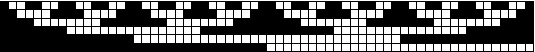
\includegraphics[width=4in]{BRGC6-cropped.pdf} 


\includegraphics[width=4in]{BCLX6-cropped.pdf} 

    \caption{Lexicographic (top), binary reflected Gray code (middle), and cool-lex (bottom) enumerations of 6-bit binary strings. \\ 
    Individual strings are read vertically with the most significant bit at the top; white is 1.
    }
    \label{binary}
\end{figure}

\section{Gray Codes for Other Objects} \label{sec:intro_Graycodes}
In this thesis, we are not concerned with counting combinatorial objects, but rather with efficiently ordering them.  We aim to create a \emph{Gray code} or \emph{minimal change ordering} for these objects.  Frank Gray's reflected binary code used complementing a single bit as the minimal change between successive binary strings in its ordering.  Other notions of minimal changes in strings are \emph{adjacent-transpositions}, or \emph{swaps}, which interchange two adjacent symbols in a string, and \emph{shifts}, in which a single symbol in a string moved to another position. Our Gray codes for strings will use a slightly more restrictive type of shift: a \emph{left-shift}, which moves a single symbol somewhere to the left within a string. 
% This means sequencing the objects such that each one differs from the other in a specific small way. For example, two successive integer strings might differ by shifting one symbol into another position, or two trees might differ by changing one node to be a child of a different node.
More specifically, if $\alpha = a_1 a_2 \ldots a_n$ is a string and $i < j$, then we let
\begin{equation}
    \lshiftindex[\alpha]{j}{i} = a_1 a_2 \ldots a_{i-1} a_j a_{i} a_{i+1} \ldots a_{j-1} a_{j+1} a_{j+2} \ldots a_n. \label{eq:leftdef}
\end{equation}


WHAT DOES IT MEAN TO HAVE A MINIMAL CHANGE ORDERING IN A TREE?

PICTURE? ESA IMAGE? BUT WITHOUT STACK?

MOVE LSHIFT DEF TO SEC 3?
NOT JUST OF THEORETICAL INTEREsT, VERY EFFICIENT


Our Gray code for ordered trees will use ``pops", which remove a node's first child, and ``pushes,'' which push one node to be the first child of another.  More specifically, the algorithm will generate trees using a pop-push operation that pops one node's first child and pushes it to become the first child of another node.  We will refer to this pop-push operation as a ``pull.''

% Our enumeration algorithms uses \emph{left shifts} and \emph{parent shifts}. Left shifts shift a single symbol in a string somewhere left (earlier) in the string; parent shifts shift a single node in a tree to be the first child of another node.

\section{Cool-Lex Order}

HAS BENEFITS OF LEX AND GRAY CODE
% connect Gray code and cool-lex order
Cool-lex order has introduced the idea of rotating sublists to enumerate languages.  Different versions of cool-lex order have been shown to enumerate several sets of combinatorial objects, including binary strings, fixed weight binary strings, Dyck words, and multiset permutations \cite{williams2009shift}.  Cool-lex orders often lead to algorithms that are faster and simpler than standard lexicographic order.  For example, the ``multicool" package in R uses a loopless cool-lex algorithm to efficiently enumerate multiset permutations.   The package started using cool-lex order for multiset permutations in versoin 1.1 and as of version 1.12 has been downloaded nearly a million times \cite{multicool_2021}.  A common thread in the cool-lex algorithms for combinatorial generation is their focus on the \emph{non-increasing prefix} of string, or the longest prefix of a string such that each successive symbol in the prefix is less than or equal to the previous symbol in the string.

\section{Goals of this Thesis}

% Cool-lex order has been shown to provide a minimal change cyclic ordering for Dyck words and binary trees. This thesis provides a new algorithm fo


This thesis will examine the use of cool-lex orders to enumerate other languages. Among these are ordered trees, Lukasiewicz words, and Motzkin words. 

This thesis will provide two primary contributions, each with sub-contributions.  

The first contribution is a `pop-push' Gray code for enumerating ordered trees in $O(1)$ time. Chapter \ref{chap:otree-graycode} will give a two-case successor rule for generating all ordered trees with $n$ nodes using at most two ``pull'' operations. Chapter \ref{chap:otree-implementation} will provide a loopless algorithm for the successor rule in \ref{chap:otree-graycode} and an implementation of the algorithm in C.

The second contribution is a shift Gray code for Lukasiewicz words.  Chapter \ref{chap:luka-graycode} will give a shift Gray code for generating Lukasiewicz words with fixed content using one prefix shift per iteration.  Chapter \ref{chap:luka-implementation} will give a loopless implementation of the algorithm in \ref{chap:luka-graycode} using an array based implementation for the special case of Motzkin words and a linked list implementation for the general case of unrestricted Lukasiewicz words.
